% !TeX root = ../../main.tex
 \resizebox{\textwidth}{\textwidth}{
     \tikzsetnextfilename{integral_image}
    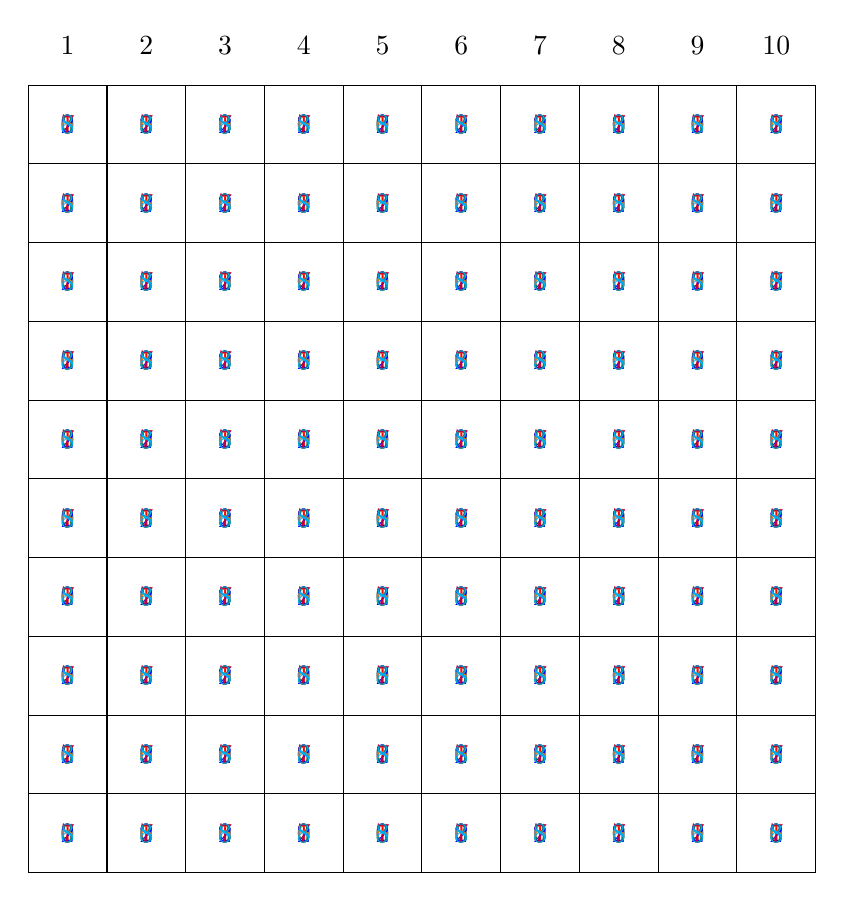
\begin{tikzpicture}
    \foreach \x in {1,...,10} {
        \draw (\x + 0.5, 11.5) node {\x};
    }
    \foreach \x in {1,...,10} {
        \foreach \y in {1,...,10} {
            \draw (\x, \y) rectangle (\x +1, \y +1);
            \ifnumcomp{\x}{<}{2}{
                \draw[color=gray] (\x +0.5, \y +0.5) node {0};
            }{
                \ifnumcomp{\x}{<}{3}{
                    \ifnumcomp{\y}{>}{2}{
                        \draw[color=gray] (\x +0.5, \y +0.5) node {0};
                    }{
                        \draw[color=red] (\x +0.5, \y +0.5) node {1};
                    }
                }{
                    \ifnumcomp{\y}{>}{7}{
                        \draw[color=gray] (\x +0.5, \y +0.5) node {0};
                    }{
                        \ifnumcomp{\y}{>}{2}{
                            \ifnumcomp{\x}{<}{5}{
                                \draw[color=blue] (\x +0.5, \y +0.5) node {2};
                            }{
                                \ifnumcomp{\y}{>}{5}{
                                    \draw[color=blue] (\x +0.5, \y +0.5) node {2};
                                }{
                                    \ifnumcomp{\y}{>}{3}{
                                        \draw[color=orange] (\x +0.5, \y +0.5) node {5};
                                    }{
                                        \draw[color=purple] (\x +0.5, \y +0.5) node {7};
                                    }
                                }
                            }
                        }{
                            \ifnumcomp{\x}{<}{5}{
                                \draw[color=teal] (\x +0.5, \y +0.5) node {3};
                            }{
                                \draw[color=cyan] (\x +0.5, \y +0.5) node {8};
                            }
                        }
                    }
                }
            }
        }
    }
    \end{tikzpicture}
}